\chapter{引言}{
{
\let\cleardoublepage\relax
}

\section{研究背景与意义}

在现代的计算系统和软件工程领域,标准化和封装起非常重要的作用,它可以确保各项技术和工具在各种不同的底层技术上都能正常工作。容器就是这样的技术,它可以使应用程序在不同的底层操作系统上都能保持正常运行,使应用程序具有可移植性。容器的高度标准化催生了云原生技术,它使应用程序和容器的管理可以自动化实施,降低了维护系统的负担,减少了运营支出成本,并消除了开发人员与系统运营人员之间沟通的障碍\citep{cloudnative}。

因此,容器化的软件越来越广泛地得到采用。根据 Morder Intelligence 的报告\citep{mordor2024},应用程序容器市场规模预计将从2024年的54.5亿美元增长到2028年的194.1亿美元。根据 CNCF 组织发布的 2022 年度调查报告\citep{cncf2024},79\%的企业用户正在使用容器技术,其中有44个百分点的企业用户在绝大多数生产环境的应用中使用了容器。

然而,目前容器化环境正在遭受威胁。根据 Red Hat 的调查\citep{redhat2023sec},在全球 600 名大中小型企业的专业人员中,有 67\% 报告他们因容器化集群的安全问题而降低了部署速度,有 37\% 报告他们因容器安全事件而遭受经济损失。Aqua Security 的一次实验\citep{michael2024}发现有超过350个组织和个人的容器化集群不受保护,至少有60\%被攻击者利用,横跨金融、航空航天、汽车、工业、安全等领域。攻击者正在利用容器化集群来进行加密挖矿活动、收集机密、创建后门等。在 Docker Hub 上,用于挖掘门罗币(Monero)的矿工镜像已有超过100万次拉取。因此,提升容器化环境的安全性迫在眉睫。

容器化环境中的攻击通常分五个阶段进行,以便攻击者实现其目标\citep{alshamrani2019survey, armo2024}。这五个阶段如下:

\begin{enumerate}
    \item 侦察:攻击者探测他想要攻击的目标计算机或网络。在此阶段,他们可以获取各种信息,例如镜像、部署、Pod、节点和集群的状态等\citep{mitre2024}。
    \item 立足:攻击者成功进入目标计算机或网络。攻击者可以通过错误配置的集群组件、容器上存在的已知漏洞、零日漏洞、供应链植入、访问令牌窃取\citep{oshrat2024}等方式进入集群中。
    \item 横向移动:攻击者在目标网络内移动,在避免被检测系统发现的同时,搜索目标网络的更多内部信息,同时试图达到阶段性目标。攻击者可在此阶段获取集群的机密信息和访问令牌,创建新的具有特权的容器,访问内部资源,部署攻击脚本等。
    \item 攻击:在此阶段,攻击者达到他的最终目标,例如破坏网络中的关键组件,获取目标组织的内部数据,或者进行勒索等。
    \item 清理:攻击者在此阶段清除痕迹,以免被发现。
\end{enumerate}

在上述阶段中:

\begin{itemize}
    \item 若在侦察阶段进行检测,由于该阶段的攻击通常是被动进行的,被动攻击不会修改或干扰通信,而是监听或监视传输的信息\citep{app10113874},因此难以检测。具体来说,攻击者可能会在网络上查找公开的容器、公开的代码存储库\citep{oshrat2024}、应用程序的版本等等。
    \item 若在立足阶段进行检测,则需要了解攻击者进入集群的途径。攻击者可能通过接入方式或漏洞利用的方法进入集群中\citep{7550947}。通过接入的方式进入集群时,攻击者利用在侦察阶段找到的公开的容器进入集群;或者利用公开的代码存储库,通过供应链攻击进入集群\citep{cicd}。通过漏洞利用的方法进入集群时,攻击者通过使用较旧版本的软件或零日漏洞进入集群中\citep{7550947}。因此,在该阶段进行检测和防御,需要综合使用多种手段,这超出了本文的范围。
    \item 若在攻击、清理阶段进行检测,则攻击者已达到其目标,通常为时已晚。
\end{itemize}

本文关注在横向移动阶段的检测。当立足阶段的检测和防御措施失效时,及时地检测横向移动有助于阻止攻击者进一步破坏集群,防止危害扩大。攻击者进行横向移动的方式多种多样,Microsoft 提出的威胁矩阵\citep{yossi2020threat}总结了多达 45 种技术可用于攻击容器化集群。不过,可以留意到,攻击者在容器化集群内移动时,是通过网络的方式进行移动的。因此,本文将利用网络流量数据,检测容器化环境中的横向移动行为。

\section{挑战}

容器化环境中的横向移动检测任务的挑战如下:

\begin{itemize}
    \item {容器化集群可用于检测的特征不明确。
    
    现有的横向移动检测研究通常在企业网络等非容器化环境中进行,主要针对登录记录进行研究。这些登录记录包含了源计算机、目的计算机和登录用户信息。攻击者通常通过社会工程学或 Mimikatz\citep{mimikatz} 等工具窃取内网中其他账号的登录凭据,以便移动到其他计算机上,因此便留下了相应的登录记录信息。然而,在容器化集群中,攻击者进行横向移动的手段有所不同,他们进入系统后,使用容器内的环境变量、服务账户等凭据,或利用逃逸漏洞,以便移动到其他容器或主机上\citep{oshrat2024}。因此,容器化环境中不包含可用于横向移动检测的登录信息等特征,还需要进一步发掘可用于检测的特征。
    }
    \item {横向移动检测任务的分类难度大,且样本不均衡,对高检测率和低误报率提出了高要求。

    对于横向移动,攻击者会尽可能隐藏其行为,使其难以从正常行为中区分出来。此外,大部分流量均为正常流量,仅有极少数流量为横向移动流量,因此,在检测横向移动时容易导致警报泛滥问题,过多警报容易让人变得麻木,反而导致横向移动检测没有起到应有的效果。因此,横向移动检测任务需在较低误报率的情况下,尽可能提高横向移动的检测率。
    }
\end{itemize}

\section{主要研究内容}

为了应对上述挑战,本文将进行以下研究:

\begin{itemize}
    \item 针对容器化集群可用于检测的特征不明确的问题,本文从两个方面着手分析。在网络流量特征方面,本文首先将分析横向移动的原理及其在网络流量中的表现,进行网络流量中的特征分析,并对各特征进行重要度评估。特征分析和特征重要度评估的结果将在后续模型中使用。
    \item 在网络流量的时空特性方面,本文进行了拓扑分析和特征嵌入方法研究。本文从流量的空间和时间两方面进行了研究。在流量的空间方面,本文首先将进行流量的拓扑结构分析,明确各网络流量所起的作用并进行分类;然后,本文将研究基于图机器学习的空间特征嵌入方法,为流量的每个节点生成嵌入向量。在流量的时间方面,本文将研究基于循环神经网络的时间特征嵌入方法,为流量序列生成时间嵌入向量。拓扑分析的结果和嵌入向量将在后续模型中使用。
    \item 针对横向移动检测任务的检测性能问题,本文首先利用了特征分析和拓扑分析的结果,对于少数关键的横向移动检测行为进行检测;对于大多数横向移动流量,本文将提出基于深度学习的横向移动检测模型 LMDCE,该模型由空间特征嵌入模块、时间特征嵌入模块、编码器—解码器模块和两步预测机制构成。通过该模型,本文提出的方法达到了 96.401\% 的 AUC 分数,超过了现有其他横向移动检测模型在容器化环境下的表现。
\end{itemize}

本文的研究框架如图~\ref{fig:research}~所示。

\begin{figure}[t]
    \centering
    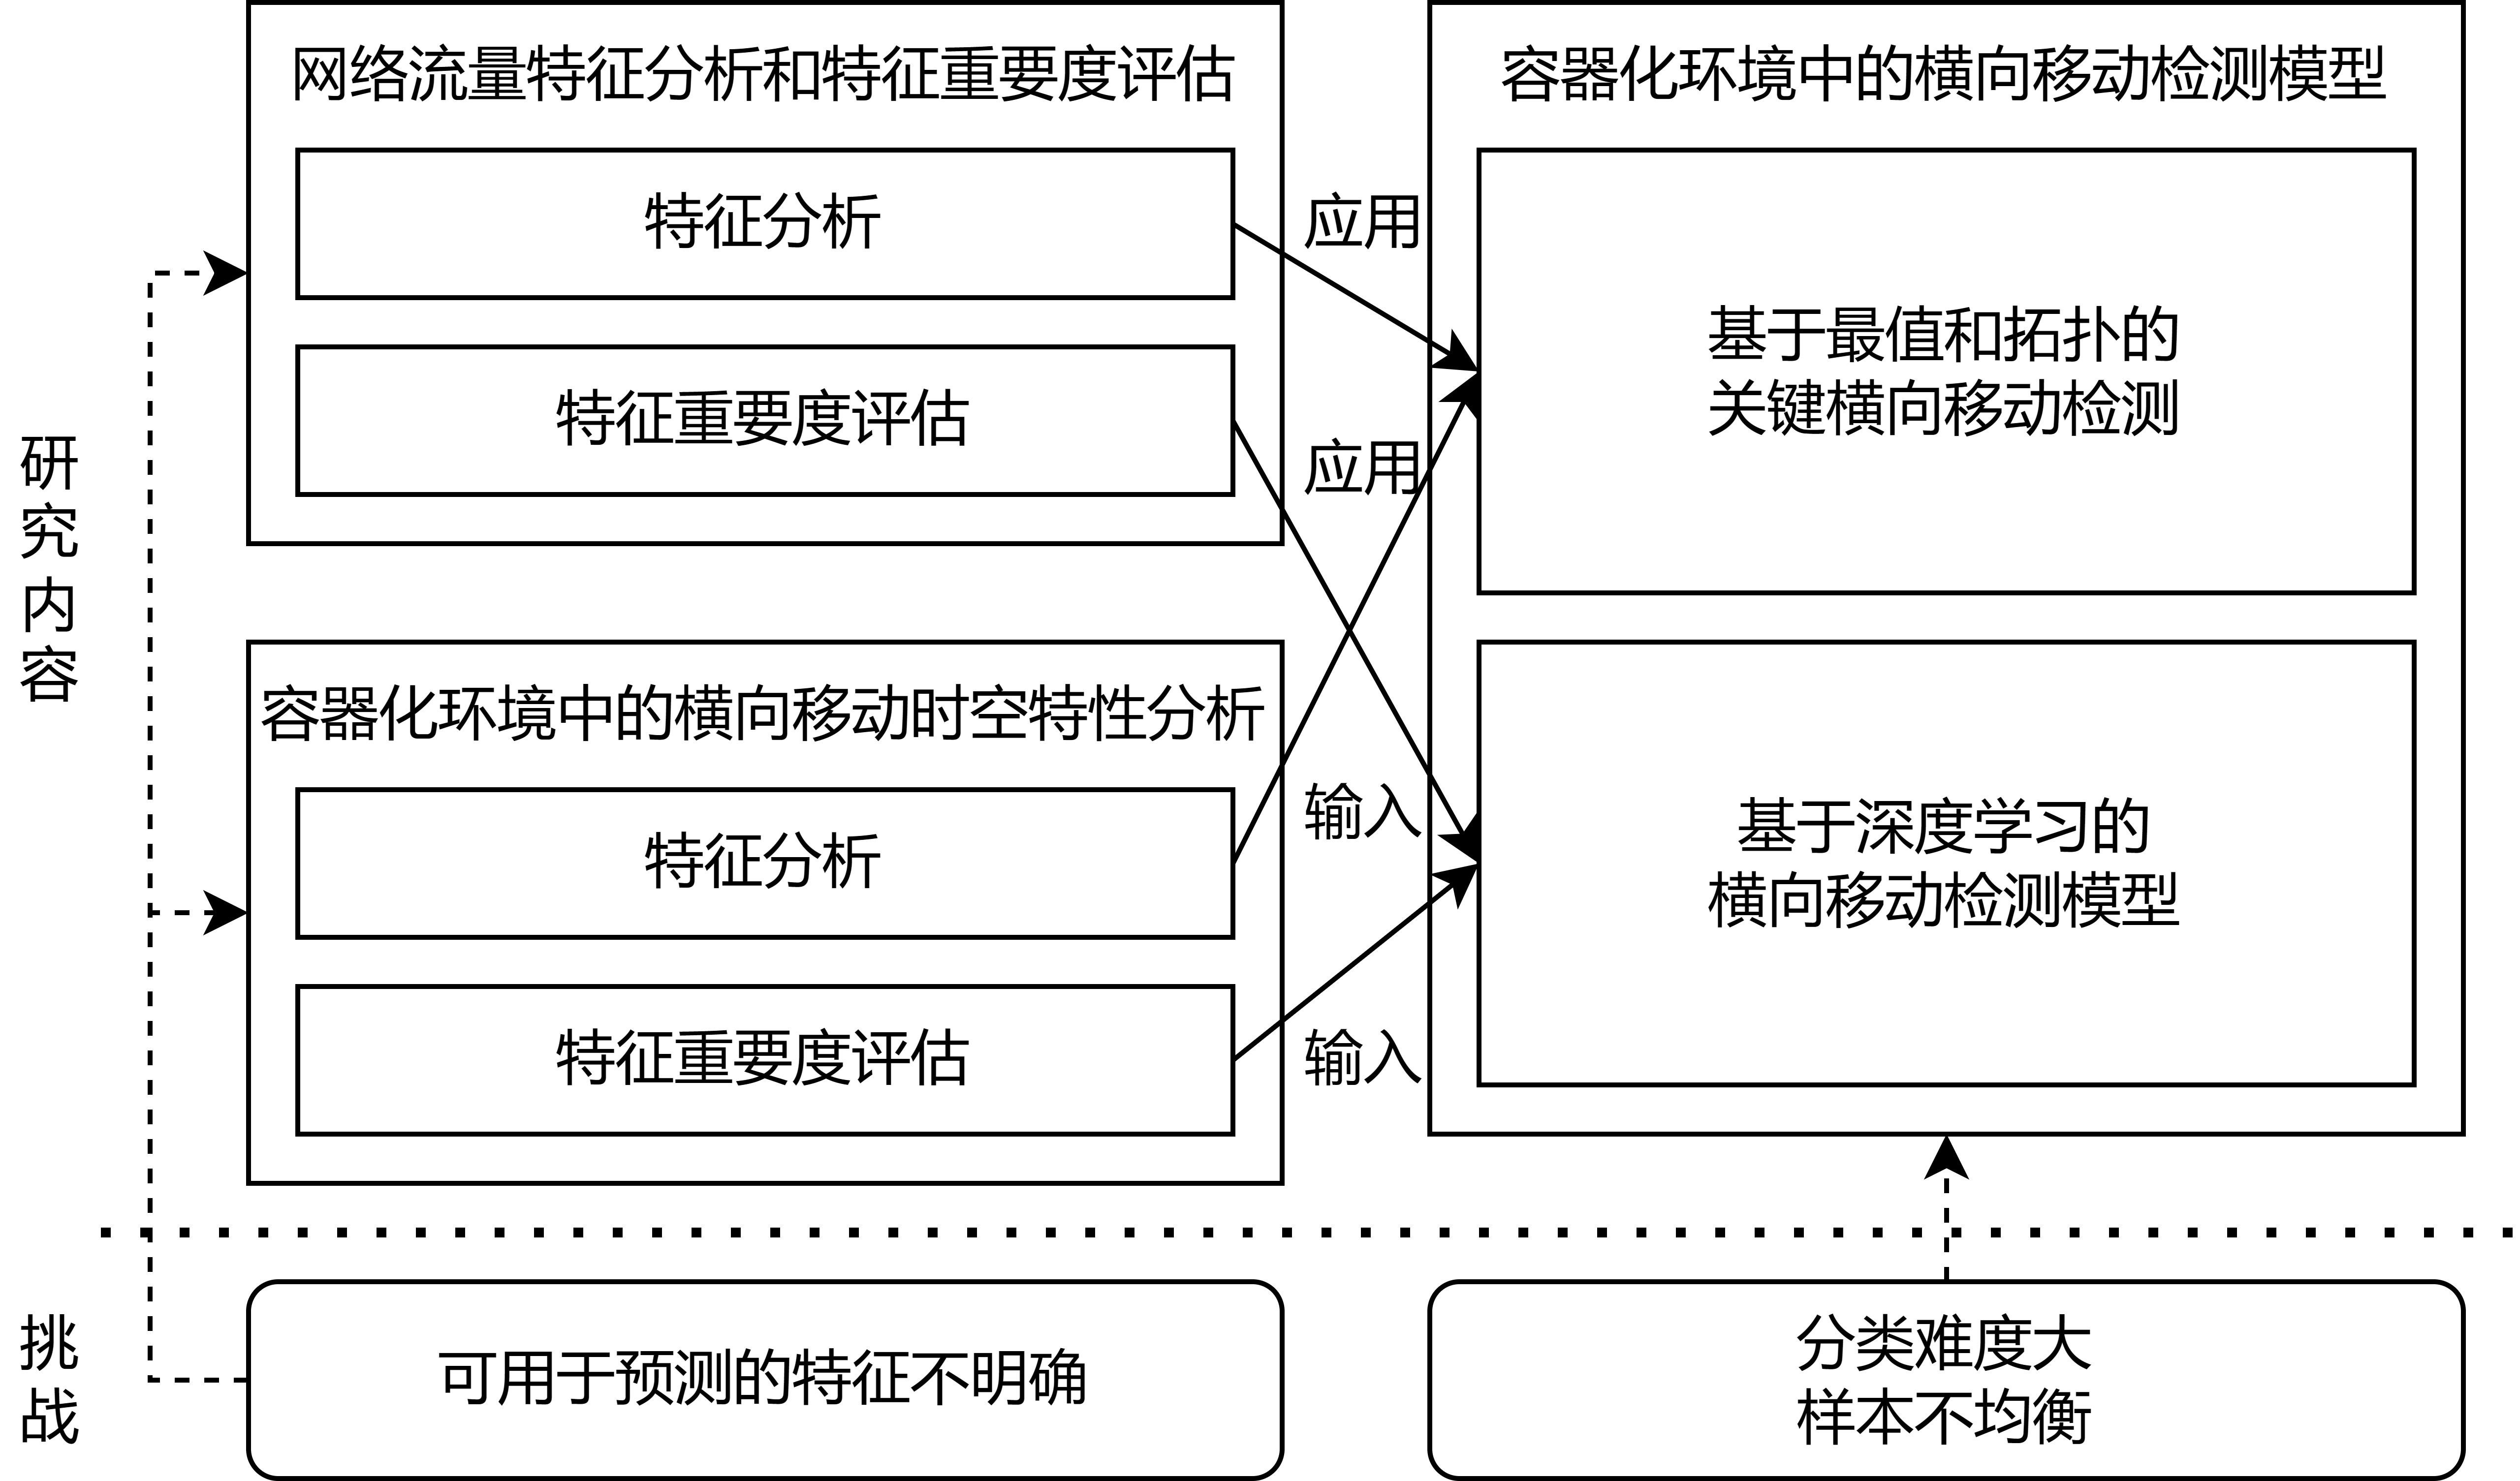
\includegraphics[width=0.8\textwidth]{research}
    \bicaption{\enspace 本文的研究框架}{\enspace The research framework of this thesis}
    \label{fig:research}
\end{figure}

\section{本文组织结构}

本文共分为六章,每章内容如下:

\begin{enumerate}
    \item 第一章:引言。该部分首先介绍了容器化环境中的横向移动检测的研究背景与意义,然后介绍了研究挑战及其对应的研究内容,最后介绍了本文组织结构。
    \item 第二章:相关研究成果与进展。该部分首先介绍了容器化环境及在该环境下存在的安全问题,然后分类介绍了现有的横向移动检测方法,指出这些方法均在非容器胡环境下应用,不能直接应用于容器化环境。接着,本文介绍了容器化环境中可行的横向移动检测技术路线。最后,介绍了本文所采用的数据集。
    \item 第三章:网络流量特征分析和特征重要度评估。首先,本文分析了容器化集群中横向移动的原理,接着通过最值分析,找到了最能体现关键的少数横向移动流量的特征,这些特征体现了横向移动导致数据传输量的变化。对于其余大部分横向移动流量,本文进行了密度分析,并采用机器学习算法进行了特征重要度评估,得到了按评估分数排列的特征列表。
    \item 第四章:容器化环境中的横向移动时空特性分析。首先,本文进行了网络流量的拓扑结构分析,指出在数据集所提供的横向移动场景中,最能体现横向移动的流量是从未与 API 服务器通信的容器开始与 API 服务器通信,同时与外部网络保持连接。接着,本文进行了空间和时间特征嵌入方法研究,分别得到了空间和时间特征嵌入向量,这些嵌入向量将作为后续检测模型的输入。
    \item 第五章:基于 Transformer 的两阶段横向移动检测方法。在第一阶段,本章首先利用了特征分析和拓扑分析的结果,提出了关键横向移动流量的检测方法。然后,在第二阶段,本章提出了一种基于 Transformer 的横向移动检测模型 LMDCE。最后,本章进行了实验,对方法和模型的各项性能进行对比验证。
    \item 第六章:总结与展望。对本文工作进行了总结,并分析了将来的研究方向。
\end{enumerate}
}